% section
\section{Experiments} \label{section::experiments}
 This section describes the experiments performed on the three implemented networks and the experimental results. The experiments were performed, to see 
 if the implemented networks are able to perform better, when changing the recurrent module with a more advanced recurrent module. The sections starts with 
 the description of the experimental setup, followed by the experimental results.
 
 % subsection
 \subsection{Experimental Setup} \label{subsection::exp_setup}
  The experiments were performed on three different datasets. Initial experiments are performed on a synthetic dataset. This has the advantage of having full 
  knowledge
  about the underlying structure of the data and that one has, in theory, an infinite amount of data for training and testing. This is a very common approach
  and performed in all papers, compared in section~\ref{section::related}.
  \\\\
  MovingMNIST is used as the synthetic dataset, which is a dataset created using handwritten digits from the famous handwritten dataset MNIST
  \cite{LeCun1998}. The idea is to use a pre-defined number of digits, which are spawned at a random position inside a given frame. Those digits are then moved 
  through the frame, given a velocity and momentum. If a digit will touch the boundary of the frame, the digit will bounce back.
  \\\\  
  The other two used datasets are real datasets\footnote{Camera images or videos from the real world.}.
  The first one is KTH \cite{Schuldt2004}, an action recognition dataset, which consists of videos where people
  do different actions, such as hand waving, running and jogging. The second one is Kitti \cite{Geiger2013}, which is an autonomous driving dataset, where
  the authors drove a car through different areas in Karlsruhe, Germany. For example through residential areas and the city.
  \\\\
  MovingMNIST is pre-processed to have a frame size of $(1 \times 64 \times 64)$, two digits per frame and ten frames per sequence.
  The training set consists of $10000$ sequences and the test set of $3000$ sequences.\\
  KTH was pre-processed to gray-scaled images and cropped to the frame size $(1 \times 80 \times 60)$.\\
  Kitti was also cropped to a specific frame size $(3 \times 160 \times 128)$.
  \\\\
  For the first experiments there are several fixed hyperparameters, simply because the network already needs several hours to train, so hyperparameter 
  optimization was not intended, because it would have blown the experiments by a wide margin.
  The amount of epochs and iterations per dataset are fixed as well, as well as using image normalization and having MSE as the
  error function for training and testing.
  \\\\
  For MovingMNIST, it was used one epoch with $5000$ iterations, for KTH $20$ epochs with $500$ iterations per epoch and for Kitti $50$ epochs with $500$ 
  iterations per epoch. The values for MovingMNIST are inspired by Elsayed et al. \cite{Elsayed2018}, where they develop a novel ConvLSTM module for PredNet and 
  train PredNet on the MovingMNIST dataset (Which is not done by the PredNet authors.).
  The values for KTH and Kitti are inspired by Lotter et al. \cite{Lotter2016}.
  In the PredNet paper the authors use $150$ epochs with $500$ iterations per epoch to train PredNet on Kitti dataset, but here the amount of epochs is reduced to
  $50$ because the training would otherwise take more then $20$ hours, which was not applicable for this thesis. Because KTH is a more \glqq simple\grqq{} dataset 
  (Only 
  objects in the scenery are moving, not the scenery as in Kitti.), the epoch size was artificially chosen to be $20$.
  \\\\
  Adam \cite{Kingma2015} was used as optimizer for all networks, always with the same learning rate of $0.001$, and the same learning rate scheduler (Dividing the 
  learning rate by factor ten after $50$\% of epochs.), even tho 
  Patraucean et al. \cite{Patraucean2015} are using RMSProp \cite{Ruder2016}, in their paper, as optimizer and a different learning rate scheduler.
  The values are used by Lotter et al. \cite{Lotter2016} for PredNet and they were chosen as the hyperparameter for this experiment.
  \\\\
  All other parameters, such as kernel-size, padding-size, channel, depth, etc. can be found in the implementation, in the yml-folder.  
  \\\\
  For the second experiments hyperparameter optimization, early stopping and used \glqq optimal values\grqq{} given by the authors in the papers was added,
  to show that using those important topics can totally change a decision.
  Due to the complexity and effort of the training of those complex neural network, it was decided to only show one example of the second experiments.
  
 % subsection
 \subsection{Experimental Results (First setup)} \label{subsection::exp_results}
  This section is divided into the three different datasets and all subsections are structured the same way. It starts by comparing the amount of paramters
  for the dataset, because the amount of parameters is directly correlated to the computing time the network needs for training and testing. It then shows
  examples of the testing output and a table of mean MSE error.
  The number of parameters directly correlates to the performance\footnote{In computer science, the performance directly correlates with the computing time.}, 
  therefore is a smaller amount always better, because the network will train faster and is also faster at test time. A tree graph of the performed experiments
  can be found in the appendix~\ref{section::appendix}.
  
  % subsubsection
  \subsubsection{MovingMNIST}
   \begin{table}[H]
    \begin{center}
     \begin{tabular}{| l | l | l |}\hline
      \textbf{Model} & \textbf{ConvLSTM} & \textbf{PredRNN} \\\hline
      Autoencoder (Depth $2$) & $537.411$ & $773.018$ \\\hline
      PredNet & $6.909.818$ & $12.421.090$ \\\hline
      Spatiotemp & $1.001.324$ & $1.415.639$ \\\hline
     \end{tabular}
    \end{center}
    \caption{Number of trainable parameter for MovingMNIST.}
   \end{table}\noindent
   We can clearly see, that the networks using PredRNN, due to it's more complex architecture, has at least $~1.41$ times the amount of parameters. In the worst
   case, here for PredNet (Because PredNet has the PredRNN module in every layer.), the value is $~1.8$. This results show, that the networks using PredRNN
   should perform better in the test to be the superior architecture, because otherwise they don't have any advantage to the architecture using ConvLSTM.
   \begin{figure}[H]
    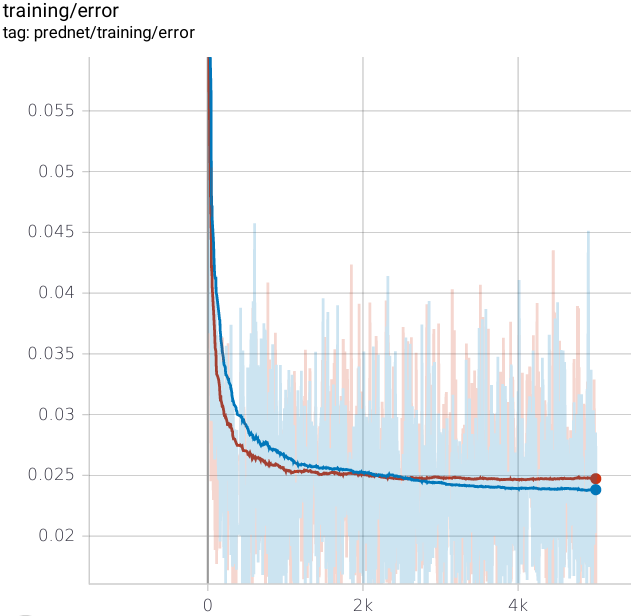
\includegraphics[width=0.45\textwidth]{../Images/prednet_mnist_training.png}
    \centering
    \caption{Training PredNet with ConvLSTM (blue) and PredRNN (red) on MovingMNIST.}
    \label{fig:prednet_mnist_training}
   \end{figure}\noindent
   \begin{figure}[H]
   \centering
   \subfloat[Ground truth]{{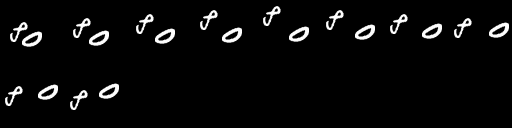
\includegraphics[width=0.6\textwidth]{../Images/prednet_mnist_groundtruth.png} }} 
   \qquad
   \subfloat[ConvLSTM]{{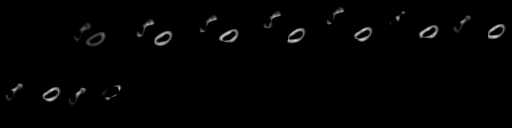
\includegraphics[width=0.6\textwidth]{../Images/prednet_mnist_convlstm_prediction.png} }} 
   \qquad
   \subfloat[PredRNN (vanished)]{{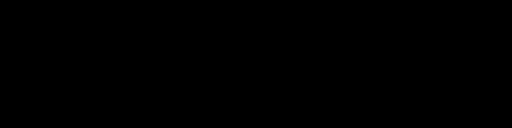
\includegraphics[width=0.6\textwidth]{../Images/prednet_mnist_predrnn_prediction.png} }}
   \caption{Test results for PredNet on MovingMNIST.}
   \label{figure::prednet_mnist_results}
  \end{figure}\noindent
  Here one can see a problem, that was always present during training. The values for MovingMNIST were vanishing very fast, which often resulted in empty images,
  for ConvLSTM and PredRNN. This is due to the fact, that PyTorch is vanishing gradients faster then Keras \cite{chollet2015}, and that Lotter et al. used 
  Matplotlib \cite{Hunter2007}, which is able to catch much smaller values then Tensorboard is (I had to multiply the values with factor ten, to even get some
  output.).
   \begin{table}[H]
    \begin{center}
     \begin{tabular}{| l | l | l |}\hline
      \textbf{Model} & \textbf{ConvLSTM} & \textbf{PredRNN} \\\hline
      Autoencoder (Depth $2$) & $0.027$ & $0.028$ \\\hline
      PredNet & $0.035$ & $0.041$ \\\hline
      Spatiotemp & $0.024$ & $0.022$ \\\hline
     \end{tabular}
    \end{center}
    \caption{Mean MSE for MovingMNIST.}
   \end{table}\noindent
   Those values directly show, that the change from ConvLSTM to PredRNN does not make any positive difference for any network performing the tests on MovingMNIST.
   Therefore, as written above, the network using PredRNN only consist of more parameter, so the choice should therefore tend to ConvLSTM, because it has less
   computing time and similar results.
   
  % subsubsection
  \subsubsection{KTH}
   \begin{table}[H]
    \begin{center}
     \begin{tabular}{| l | l | l |}\hline
      \textbf{Model} & \textbf{ConvLSTM} & \textbf{PredRNN} \\\hline
      Autoencoder (Depth $2$) & $542.531$ & $781.760$ \\\hline
      PredNet & $850.325$ & $1.285.730$ \\\hline
      Spatiotemp & $1.007.598$ & $1.421.913$ \\\hline
     \end{tabular}
    \end{center}
    \caption{Number of trainable parameter for KTH.}
   \end{table}\noindent
   \begin{figure}[H]
   \centering
   \subfloat[Ground truth]{{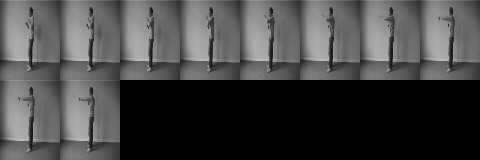
\includegraphics[width=0.6\textwidth]{../Images/prednet_kth_groundtruth.png} }} 
   \qquad
   \subfloat[ConvLSTM]{{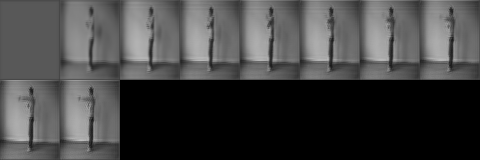
\includegraphics[width=0.6\textwidth]{../Images/prednet_kth_convlstm.png} }} 
   \qquad
   \subfloat[PredRNN]{{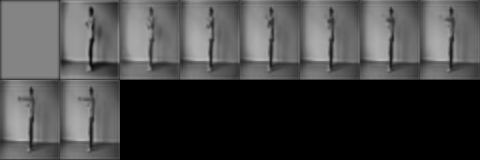
\includegraphics[width=0.6\textwidth]{../Images/prednet_kth_predrnn.png} }}
   \caption{Test results for PredNet on KTH.}
   \label{figure::prednet_kth_results}
  \end{figure}\noindent
   \begin{table}[H]
    \begin{center}
     \begin{tabular}{| l | l | l |}\hline
      \textbf{Model} & \textbf{ConvLSTM} & \textbf{PredRNN} \\\hline
      Autoencoder (Depth $2$) & $1.55e-3$ & $0.05$ (didn't converged) \\\hline
      PredNet & $1.95e-3$ & $1.93e-3$ \\\hline
      Spatiotemp & $3.1e-3$ & $0.025$ (didn't converged) \\\hline
     \end{tabular}
    \end{center}
    \caption{Mean MSE for KTH.}
   \end{table}
  
  % subsubsection
  \subsubsection{Kitti}
   \begin{table}[H]
    \begin{center}
     \begin{tabular}{| l | l | l |}\hline
      \textbf{Model} & \textbf{ConvLSTM} & \textbf{PredRNN} \\\hline
      Autoencoder (Depth $2$) & $542.531$ & $781.760$ \\\hline
      PredNet & $8.222.559$ & $12.430.626$ \\\hline
      Spatiotemp & $1.640.321$ & $2.200.641$ \\\hline
     \end{tabular}
    \end{center}
    \caption{Number of trainable parameter for Kitti.}
   \end{table}\noindent
   \begin{figure}[H]
   \centering
   \subfloat[Ground truth]{{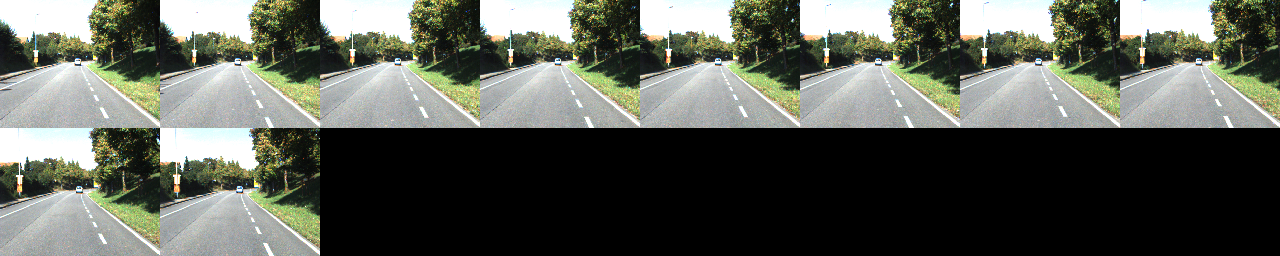
\includegraphics[width=0.7\textwidth]{../Images/prednet_kitti_groundtruth.png} }} 
   \qquad
   \subfloat[ConvLSTM]{{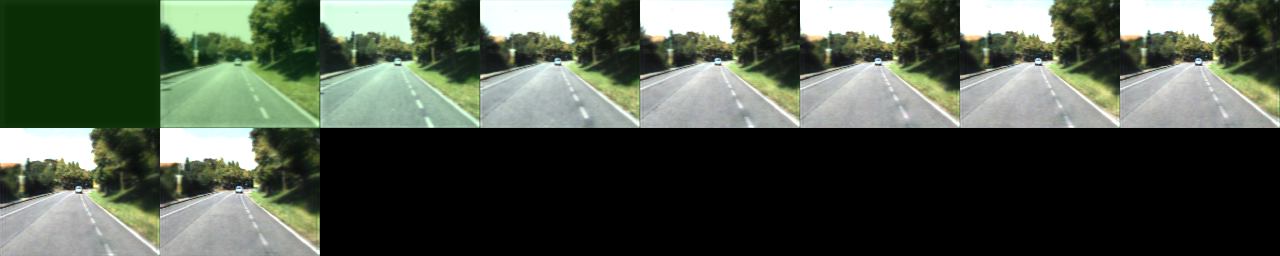
\includegraphics[width=0.7\textwidth]{../Images/prednet_kitti_convlstm.png} }} 
   \qquad
   \subfloat[PredRNN]{{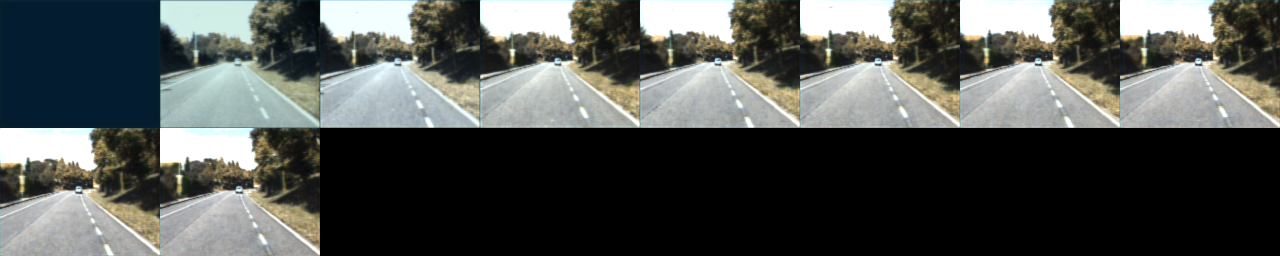
\includegraphics[width=0.7\textwidth]{../Images/prednet_kitti_predrnn.png} }}
   \caption{Test results for PredNet on Kitti.}
   \label{figure::prednet_kth_results}
  \end{figure}\noindent
   \begin{table}[H]
    \begin{center}
     \begin{tabular}{| l | l | l |}\hline
      \textbf{Model} & \textbf{ConvLSTM} & \textbf{PredRNN} \\\hline
      Autoencoder (Depth $2$) & $0.02$ & $0.013$ \\\hline
      PredNet & $0.019$ & $0.02$ \\\hline
      Spatiotemp & $0.018$ & $0.017$ \\\hline
     \end{tabular}
    \end{center}
    \caption{Mean MSE for Kitti.}
   \end{table}\noindent
 \\\\
 The experiments showed, that using this kind of setup, the PredRNN as recurrent module does not lead to a significant performance boost, but instead only
 increases the number of trainable parameter. Therefore, using this setup, PredRNN is not the superior sub-module and should not be used. But, as this experiments
 are performed without any kind of hyperparameter optimization, this results are not valid to make a real decision if PredRNN is really not superior to the 
 standard ConvLSTM module.

 % subsection
 \subsection{Experimental Results (Second setup)} \label{subsection::second_exp}
  This test was only performed on the KTH dataset, with an optimal learning rate of $0.0001$ for the Autoencoder.
  \begin{figure}[H]
   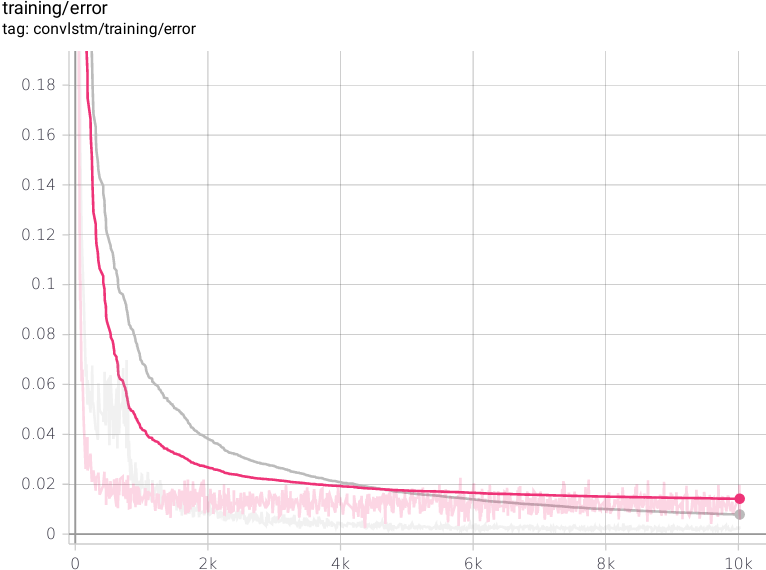
\includegraphics[width=0.6\textwidth]{../Images/exp2_training_error.png}
   \centering
   \caption{Training Autoencoder with ConvLSTM (red) and PredRNN (gray) on KTH using hyperparameter optimization and early stopping.}
   \label{fig:autoenc_exp2_training}
  \end{figure}\noindent
  The mean test mse error for the Autoencoder using the standard ConvLSTM module is: $0.0013$ and for the Autoencoder using the PredRNN module: $0.00072$.
  This means, that PredRNN was able to boost the performance of the Autoencoder by more then $80$ percent.
  \begin{figure}[H]
   \centering
   \subfloat[Ground truth]{{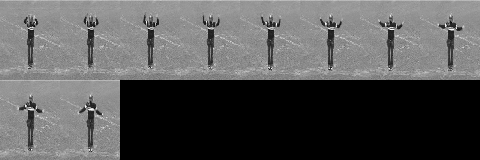
\includegraphics[width=0.65\textwidth]{../Images/exp2_test_ground.png} }} 
   \qquad
   \subfloat[ConvLSTM]{{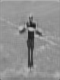
\includegraphics[width=0.1\textwidth]{../Images/exp2_test_convlstm.png} }} 
   \qquad
   \subfloat[PredRNN]{{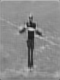
\includegraphics[width=0.1\textwidth]{../Images/exp2_test_predrnn.png} }}
   \caption{Test results for Autoencoder on KTH using hyperparameter optimization and early stopping.}
   \label{figure::prednet_mnist_results}
  \end{figure}\noindent
  This experiment showed the importance of hyperparameter optimization and early stopping and why it should be used always in terms of learning neural networks.
  A more explicit analysis of this result is given in the discussion~\ref{section::discussion}.